\documentclass[journal]{IEEEtran}
\usepackage[a5paper, margin=10mm]{geometry}
%\usepackage{lmodern} % Ensure lmodern is loaded for pdflatex
\usepackage{tfrupee} % Include tfrupee package


\setlength{\headheight}{1cm} % Set the height of the header box
\setlength{\headsep}{0mm}     % Set the distance between the header box and the top of the text


%\usepackage[a5paper, top=10mm, bottom=10mm, left=10mm, right=10mm]{geometry}

%
\setlength{\intextsep}{10pt} % Space between text and floats

\makeindex


\usepackage{cite}
\usepackage{amsmath,amssymb,amsfonts,amsthm}
\usepackage{algorithmic}
\usepackage{graphicx}
\usepackage{textcomp}
\usepackage{xcolor}
\usepackage{txfonts}
\usepackage{listings}
\usepackage{enumitem}
\usepackage{mathtools}
\usepackage{gensymb}
\usepackage{comment}
\usepackage[breaklinks=true]{hyperref}
\usepackage{tkz-euclide} 
\usepackage{listings}
\usepackage{multicol}
\usepackage{xparse}
\usepackage{gvv}
%\def\inputGnumericTable{}                                 
\usepackage[latin1]{inputenc}                                
\usepackage{color}                                            
\usepackage{array}                                            
\usepackage{longtable}                                       
\usepackage{calc}                                             
\usepackage{multirow}                                         
\usepackage{hhline}                                           
\usepackage{ifthen}                                               
\usepackage{lscape}
\usepackage{tabularx}
\usepackage{array}
\usepackage{float}
\usepackage{ar}
\usepackage[version=4]{mhchem}


\newtheorem{theorem}{Theorem}[section]
\newtheorem{problem}{Problem}
\newtheorem{proposition}{Proposition}[section]
\newtheorem{lemma}{Lemma}[section]
\newtheorem{corollary}[theorem]{Corollary}
\newtheorem{example}{Example}[section]
\newtheorem{definition}[problem]{Definition}
\newcommand{\BEQA}{\begin{eqnarray}}
\newcommand{\EEQA}{\end{eqnarray}}

\theoremstyle{remark}


\begin{document}
\bibliographystyle{IEEEtran}
\onecolumn

\title{12.353}
\author{INDHIRESH S- EE25BTECH11027}
\maketitle


\renewcommand{\thefigure}{\theenumi}
\renewcommand{\thetable}{\theenumi}

\textbf{Question}. Which one of the following describes the relationship among the three vectors
\begin{align*}
    \hat{i}+\hat{k}+\hat{k},2\hat{i}+3\hat{j}+\hat{k},5\hat{i}+6\hat{j}+4\hat{k}
\end{align*}
\begin{enumerate}
    \item The vectors are mutually perpendicular
    \item The vectors are linearly dependent
    \item The vectors are linearly independent
    \item The vectors are unit vectors
\end{enumerate}
\textbf{Solution}:\\
Let us solve the given equation theoretically and then verify the solution computationally.\\
Let
\begin{align}
\Vec{A}=\myvec{1\\1\\1}\;\;\Vec{B}=\myvec{2\\3\\1}\;\;and\;\;\myvec{5\\6\\4}
\end{align}
Let 
\begin{align}
   \Vec{M}=\myvec{\Vec{A}&\Vec{B}&\Vec{C}}
\end{align}

\begin{align}
    \Vec{M}=\myvec{1&2&5\\1&3&6\\1&1&4}
\end{align}
Now applying row operations\\
$R_2\longrightarrow R_2-R_1$ and \\
$R_3\longrightarrow R_3-R_1$
\begin{align}
   \myvec{1&2&5\\1&3&6\\1&1&4}=\myvec{1&2&5\\0&1&1\\0&-1&-1}
\end{align}
Now doing row operation\\
$R_3\longrightarrow R_3+R_2$
\begin{align}
   \myvec{1&2&5\\0&1&1\\0&-1&-1}= \myvec{1&2&5\\0&1&1\\0&0&0}
\end{align}
Here the rank of the matrix is 2.\\
Since the rank is less than the number of vectors , the vectors are linearly dependent

\begin{figure}[h]
    \centering
    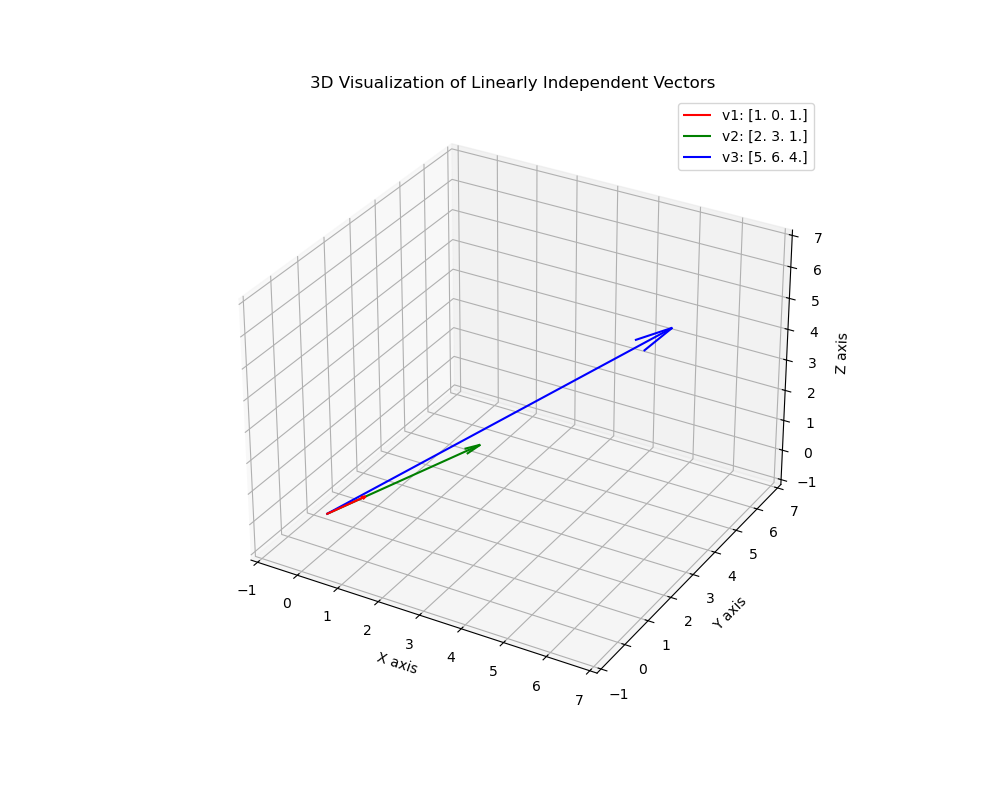
\includegraphics[height=0.5\textheight, keepaspectratio]{figs/figure1.png}
    \label{figure_1}
\end{figure}

\end{document}